% Created 2021-01-24 Sun 23:24
% Intended LaTeX compiler: pdflatex
\documentclass[11pt]{article}
\usepackage[utf8]{inputenc}
\usepackage[T1]{fontenc}
\usepackage{graphicx}
\usepackage{grffile}
\usepackage{longtable}
\usepackage{wrapfig}
\usepackage{rotating}
\usepackage[normalem]{ulem}
\usepackage{amsmath}
\usepackage{textcomp}
\usepackage{amssymb}
\usepackage{capt-of}
\usepackage{hyperref}
\usepackage{minted}
\hypersetup{colorlinks=true, linkcolor=black, filecolor=red, urlcolor=blue}
\usepackage[turkish]{babel}
\author{Eren Hatırnaz}
\date{10 Kasım 2020}
\title{.NET 5.0 sürümü yayınlandı\\\medskip
\large 10 Kasım 2020}
\hypersetup{
 pdfauthor={Eren Hatırnaz},
 pdftitle={.NET 5.0 sürümü yayınlandı},
 pdfkeywords={},
 pdfsubject={},
 pdfcreator={Emacs 27.1 (Org mode 9.3)},
 pdflang={Turkish}}
\begin{document}

\maketitle
\tableofcontents \clearpage\shorthandoff{=}

\begin{center}
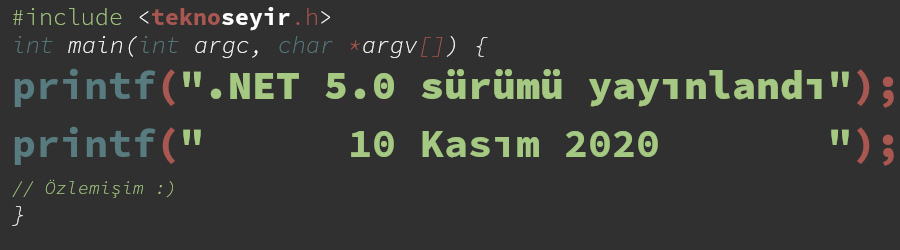
\includegraphics[width=.9\linewidth]{gorseller/yazilim-gundemi-banner.png}
\end{center}

Geçtiğimiz sene düzenli olarak yazmaya çalıştığım \href{../../../README.org}{Yazılım Gündemi yazılarını}
takip etmiş arkadaşlar .NET Framework ve .NET Core projelerinin artık tek bir
isim altında ".NET 5.0" olarak devam edeceği haberini (bkz: \href{../../2019/22/yazilim-gundemi-22.pdf}{Yazılım Gündemi - 22})
hatırlayacaklardır. İşte o gün geldi. Bugün Microsoft, \href{https://devblogs.microsoft.com/dotnet/announcing-net-5-0/}{.NET 5.0 sürümünü
yayınladı}.

.NET SDK'sının bu sürümüyle birlikte C\# 9 ve F\# 5 sürümleri de hayatımıza girmiş
bulunuyor. Visual Basic de SDK içerisinde mevcut fakat daha önceden de haberini
yaptığım (bkz: \href{../../2020/10/yazilim-gundemi-2020-10.pdf}{Yazılım Gündemi - 2020/10}) gibi artık geliştirilmeye devam
edilmediği için dil değişikliği içermiyor. Visual Basic Application Framework
tarafında birkaç iyileştirilme yapılmış o kadar. Visual Studio kullanıcılarının
.NET 5.0'ı kullanabilmesi için \href{https://visualstudio.microsoft.com/}{Visual Studio 16.8} ya da daha üstü bir sürüme
ihtiyaçları var. \href{https://code.visualstudio.com/}{Visual Studio Code} kullanıcıları için ise \href{https://code.visualstudio.com/docs/languages/dotnet}{C\# eklentisi} zaten
hali hazırda C\# 9'u destekliyormuş.

Ayrıca bir sonraki .NET sürümü 6.0 için de şimdiden tarih verilmiş: Kasım 2021.
Bundan sonra her Kasım ayında yeni bir büyük .NET sürümü gelecek diye de not
düşmüşler. .NET 5.0 sürümü, .NET 6.0 sürümü yayınlandıktan 3 ay sonrasına kadar
(Şubat 2022) desteklenmeye devam edilecek.

.NET Core'dan alışık olan arkadaşlar yadırgamayacaklardır (zaten uzun zamandır
kullandıkları için) fakat .NET Framework kullanıcıları için ilginç bir gelişme
olarak .NET 5.0 sürümü Windows, MacOS ve Linux tabanlı işletim sistemlerininde
ve x86, x64, Arm32 ve Arm64 mimarilerinde destekli şekilde geliyor. Desteklenen
tüm işletim sistemi ve mimariler için \href{https://github.com/dotnet/core/blob/master/release-notes/5.0/5.0-supported-os.md}{şu sayfayı inceleyebilirsiniz}.

Şimdi bu sürümle birlikte gelen birkaç gelişmeye göz atalım isterseniz. Özellik
başlıklarını Türkçe'ye çevirince anlam kaybı olduğu için İngilizce şekilde
kullanacağım.

\section{Top-level programs}
\label{sec:org3f58a6f}
C\# ve diğer dillerden alışık olduğumuz yapının aksine artık C\# 9.0 ile
birlikte Python ve diğer betik dillerindeki gibi şu şekilde kod
yazabileceğiz:
\begin{minted}[breaklines=true,breakanywhere=true,frame=lines, linenos, label=C\#]{csharp}
using System;

var ad = "Eren";
var soyad = "Hatirnaz";
var suan = DateTime.Now;

Console.WriteLine($"Merhaba {ad} {soyad}!");
Console.WriteLine($"Guncel tarih-saat: {suan}");
\end{minted}
Yani artık \texttt{main} fonksiyonu tanımlamaya gerek yok. Daha gelişmiş bir örnek
için \href{https://github.com/dotnet/iot/tree/master/samples/led-blink}{burayı inceleyebilirsiniz}.
\section{Records}
\label{sec:org244e496}
Records için aslında yeni bir class türü diyebiliriz. Basit objeler
tanımlamak için gerçekten ideal bir yapı sunuyor. Şöyle ki:
\begin{minted}[breaklines=true,breakanywhere=true,frame=lines, linenos, label=C\#]{csharp}
public record Kisi (string Ad, string Soyad, string Meslek, int Yas)
\end{minted}
şeklinde tek bir satırda sınıfınızı tanımlayıp sonra da onu bu şekilde
kullanabiliyorsunuz:
\begin{minted}[breaklines=true,breakanywhere=true,frame=lines, linenos, label=C\#]{csharp}
var eren = new Kisi {
    Ad = "Eren",
    Soyad = "Soyad",
    Meslek = "Back-End Developer",
    Yas = 25
};
\end{minted}
Bu tarz basit tanımlamalar için oldukça sade bir kullanım sunuyor bence.
\section{Logical and property patterns}
\label{sec:org4bd9c4e}
Artık kontrol ifadelerimizi daha okuma diline yakın bir şekilde bu şekilde
yazabileceğiz:
\begin{minted}[breaklines=true,breakanywhere=true,frame=lines, linenos, label=C\#]{csharp}
Console.WriteLine("Programdan cikmak istiyor musunuz? (e/H): ");
var kullanici_tercihi = Console.ReadKey();

if (kullanici_tercihi.KeyChar is 'E' or 'e')
{
    System.Environment.Exit(0);
}
\end{minted}
\section{Windows Forms designer güncellendi}
\label{sec:orgd174c2b}
\begin{center}
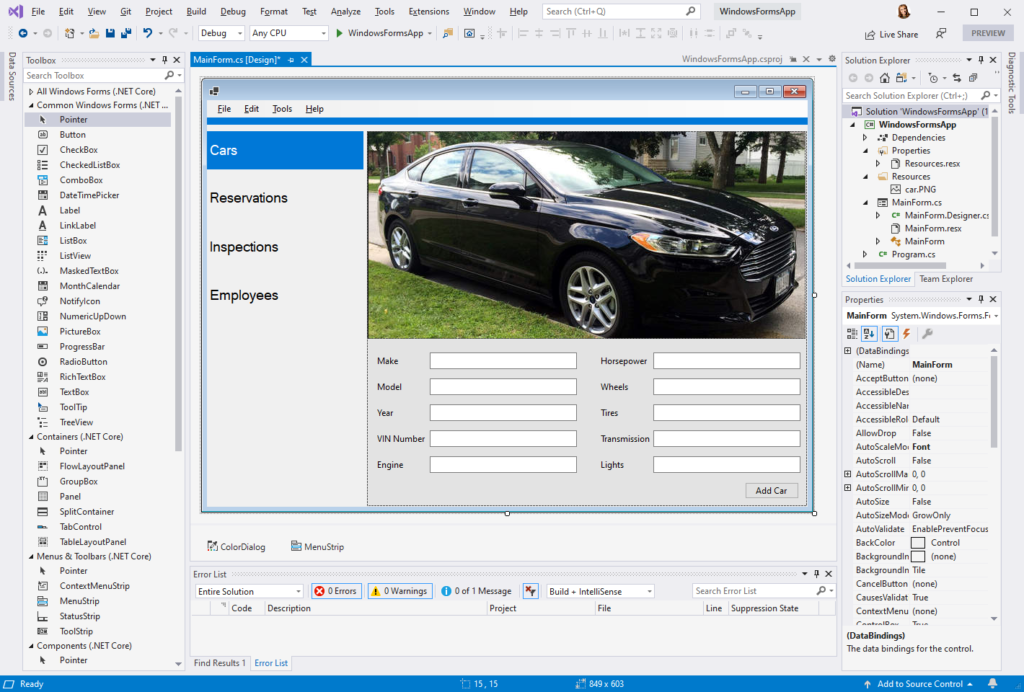
\includegraphics[width=.9\linewidth]{gorseller/winforms-designer.png}
\end{center}

Visual Studio 16.8 sürümüyle birlikte içerisindeki Windows Form tasarlayıcı
aracı de güncellenmiş. Artık tüm Windows Forms ve Telerik komponentlerini
destekliyormuş. Bu zaten yıllardır Visual Studio içerisinde olan bir özellik
değil mi? Ben uzun zamandır Microsoft teknolojilerinden uzak kaldığım için
(ben en son .NET yazarken dolar 1.7 falandı :D) gelişmeleri o kadar net
bilmiyorum. Neden bu yenilik olarak yazıya eklenmiş. Bilen arkadaşlar
aydınlatsın beni lütfen.
\section{Single file applications}
\label{sec:org181485d}
İsminden de kolayca anlaşılabileceği gibi bu özellikle birlikte artık
uygulamalarınızı tek bir çalıştırılabilir (executable) haline getirip,
kullanıcılarınıza daha kolay bir şekilde ulaştırabileceksiniz. Bu özellik .NET
Core 3.1 sürümüyle birlikte gelmişti fakat bu sürümle birlikte çalışma
mantığıyla ilgili bazı değişiklikler yaparak çeşitli performans
iyileştirmelerine gitmişler. İsmi bana son senelerde web tarafında çokça
popülerleşen "\href{https://en.wikipedia.org/wiki/Single-page\_application}{Single Page Application}" yaklaşımını hatırlattı :).

Oluşturabileceğiniz iki çeşit Single File Application var. Birisi framework'e
bağımlı (kullanıcının bilgisayarında .NET 5.0 Runtime kurulu olmak zorunda)
uygulama, diğeri de tamamen kendi başına çalışabilir uygulama. Tamamen kendi
başına çalışabilen SFA içerisinde çalışması için gerekli araç setini ve tüm
bağımlılıklarını içerdiği için boyutu büyük olacaktır. Yazdığınız bir programı
SFA şeklinde paylaşmak için şu komutları kullanabiliyorsunuz:

\begin{itemize}
\item Framework bağımlı: \texttt{dotnet publish -r linux-x64 -{}-self-contained false
     /p:PublishSingleFile=true}
\item Tamamen kendi başına çalışan \texttt{dotnet publish -r linux-x64 -{}-self-contained
     true /p:PublishSingleFile=true}
\end{itemize}
\section{Son sözler ve ileri okuma önerileri}
\label{sec:org4aa2b9b}
Yazılım Gündemi yazıları yazmayı bitirdikten uzun bir zaman sonra ilk defa
oturup tekrar böyle bir yazı kaleme alabildim. Açıkcası özlemedim desem yalan
olur ama maalesef artık yazılım gündemini eskisi kadar sık takip edemiyorum.

Her neyse fazla nostalji duygusuna girmeden bu yazıyı da burada noktalamış
olayım. Elimden geldiği ölçüde yayınlanan blog yazısı üzerinden dikkatimi
çeken ve anlayabildiğim özellik ve değişiklikleri sizlere aktarmaya çalıştım.
Diğer özellikler ve değişiklikler için Microsoft'un blogunda \href{https://devblogs.microsoft.com/dotnet/announcing-net-5-0/}{yayınlanan
detaylı yazıyı} okumanızı şiddetle tavsiye ederim. Eğer yanlış değerlendirdiğim
ya da doğru hatırlamadığım kısımlar varsa lütfen beni düzeltmekten kendinizi
geri koymayın.

Microsoft'un bugün yayınladığı .NET 5.0 sürüm hakkında siz ne düşünüyorsunuz?
Özellikle .NET teknolojilerinde aktif çalışan arkadaşların bu sürüm hakkında
yorumlarını okumayı çok isterim. Aktif projelerinizi hemen geçirmezsiniz büyük
ihtimal ama yeni projelerde bunu tercih eder misiniz? Artıları ve eksileri
nelerdir? "Şu sorunuma derman olacak özellikler geldi" dediğiniz bir şey var
mı? Tüm bu soruları -dilerseniz- aşağıdaki yorumlar bölümünde
cevaplayabilirsiniz.

\href{https://gist.github.com/richlander/50c34a8714eb3436e5d9d4d5d420776e}{.NET kod örnekleri için buraya tıklayabilirsiniz}.

\textbf{\textbf{İleri Okuma Önerileri}}
\begin{itemize}
\item \href{https://devblogs.microsoft.com/dotnet/performance-improvements-in-net-5/}{Performance Improvements in .NET 5 | .NET Blog}
\item \href{https://devblogs.microsoft.com/dotnet/Arm64-performance-in-net-5/}{ARM64 Performance in .NET 5 | .NET Blog}
\item \href{https://devblogs.microsoft.com/aspnet/grpc-performance-improvements-in-net-5/}{gRPC performance improvements in .NET 5 | ASP.NET Blog}
\item \href{https://devblogs.microsoft.com/dotnet/introducing-c-source-generators/}{Introducing C\# Source Generators | .NET Blog}
\end{itemize}
\section{Lisans}
\label{sec:orgf3edcd3}
\begin{center}
\begin{center}

\includegraphics[height=1.5cm]{../../../img/CC_BY-NC-SA_4.0.png}
\end{center}

\href{dotnet-5-0.org}{.NET 5.0 sürümü yayınlandı} yazısı \href{https://erenhatirnaz.github.io}{Eren Hatırnaz} tarafından \href{http://creativecommons.org/licenses/by-nc-sa/4.0/}{Creative Commons
Atıf-GayriTicari-AynıLisanslaPaylaş 4.0 Uluslararası Lisansı} (CC BY-NC-SA 4.0)
ile lisanslanmıştır.
\end{center}
\end{document}
